\section{Points and Lines}

\begin{frame}{}
  \begin{center}
    {\bf Part I: Points and Lines}
  \end{center}
\end{frame}

\begin{frame}{What are Computational Geometry Problems?}

  Computational Geometry problems involve the calculation of structures such as:
  \begin{itemize}
    \item Points;
    \item Lines;
    \item Circles;
    \item Triangles and Squares;
    \item General Poligons;
  \end{itemize}\bigskip

  They can be very fun, but they are also a but troublesome to program.

  Make sure to try the practice problems!

\end{frame}


\begin{frame}[t]{Example Geometry Problem}

  \begin{columns}
  \column{0.45\textwidth}
  \begin{block}{}
    {\bf Input:} $N$ rectangles, described as $\{x, y, w, h\}$.\\
    {\bf Output:} Shortest length of axis-aligned lines to connect all rectangles;
  \end{block}

  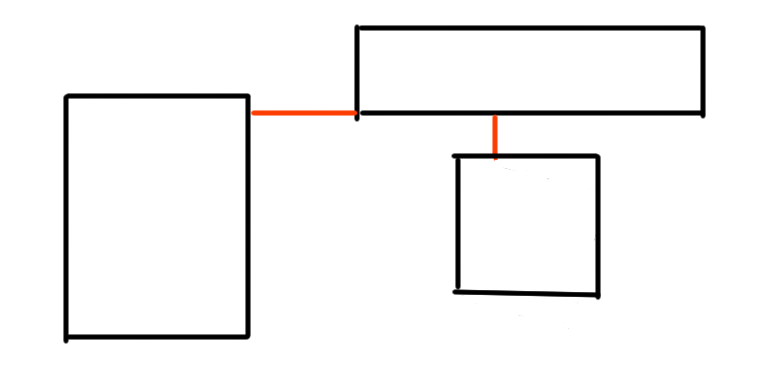
\includegraphics[width=1\textwidth]{img/sampleproblem_2.png}
  \column{0.5\textwidth}
  How to solve?
  \begin{itemize}
    \item Calculate the axis aligned distance between every pair of rectangles.
    \begin{itemize}
      \item Break the rectangle in 4 points;
      \item Calculate distance between point and segment;
    \end{itemize}
    \item Transform data into a graph;
    \item Use Minimum Spanning Tree to calculate Distance;
  \end{itemize}
\end{columns}
\end{frame}

% Special cases
\begin{frame}{Be careful of special cases}
  Geometry problems usually have special cases. It is important to test your
  algorithm on paper before programming!\bigskip

  \begin{itemize}
    \item Multiple points in the same position;
    \item Collinear points (three points in the same line);
    \item Vertical lines (bad tangent value, division by 0);
    \item Parallel Lines (bad intersection value);
    \item Intersection at end of a segment;
    \item etc;
  \end{itemize}
\end{frame}

% Precision Errors
\begin{frame}[fragile]{Avoiding Precision Errors}
  Geometry problems frequently require working with floating point numbers.
  Follow these hints to avoid precision errors:\bigskip

  \begin{itemize}
    \item If possible, work with integers.
    \begin{itemize}
      \item Try to do the floating point operations last, if possible.
    \end{itemize}
    \item Use the Long Double data type;
    \item Use the following code for equality comparison:
\begin{verbatim}
if (float_1 == float_2)               // Wrong!
if (fabs(float_1 - float_2) < EPS)    // Correct!
                                      // EPS = 10^-9
\end{verbatim}
    \item Reduce the number of floating point operations.
    \begin{itemize}
      \item Example: Instead of a/b/c, use a/(b*c);
    \end{itemize}
  \end{itemize}
\end{frame}

\subsection{Points}
\begin{frame}[fragile]{Data Structure for Point}
  \begin{columns}
    \column{0.2\textwidth}
    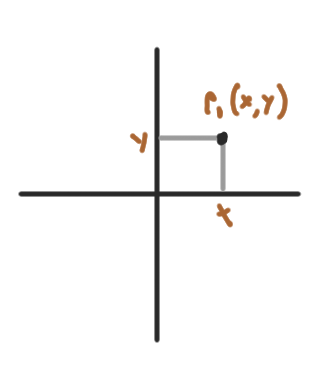
\includegraphics[width=\textwidth]{../img/geom2}
    \column{0.8\textwidth}
    \begin{exampleblock}{}
\begin{verbatim}
struct point_i {
  int x, y;  // integer coordinates
  point_i() { x = y = 0; }
  point_i(int _x, int _y) : x(_x), y(_y) {}
};

struct point {
  double x, y; // double coordinates
  point() { x = y = 0.0;}
  point(double _x, double _y) : x(_x), y(_y) {}
};
\end{verbatim}
    \end{exampleblock}
  \end{columns}
\end{frame}

\begin{frame}[fragile]{Overloading Point Operators}{Allows sorting points with "sort()"}

    \begin{exampleblock}{}
      {\smaller
\begin{verbatim}
struct point { double x, y;
   point() { x = y = 0.0;
   point(double _x, double _y) : x(_x), y(_y) {}

   bool operator < (point other) const {           // Overloading "<"
      if (fabs(x - other.x) > EPS)
         return x < other.x;
      return y < other.y; }
   bool operator == (point other) const {          // Overloading "=="
      return (fabs(x - other.x) < EPS &&
             (fabs(y - other.y) < EPS)); }
   }

point a = point(1,2); point b = point(3,4);

if (!(a == b)) printf("Different\n");
\end{verbatim}}
    \end{exampleblock}
\end{frame}

\begin{frame}[fragile]{Point Distance}
    \begin{exampleblock}{}
{\smaller
\begin{verbatim}
// Euclidean Distance: "normal" distance
#define hypot(dx,dy) sqrt(dx*dx + dy*dy)
double dist(point p1, point p2) { return hypot(p1.x - p2.x, p1.y - p2.y); }

// Taxicab Distance / Manhattan Distance : Distance on a grid
double taxicab(point p1, point p2) { return fabs(p1.x-p2.x) + fabs(p1.y-p2.y); }
\end{verbatim}}
    \end{exampleblock}

    \begin{center}
      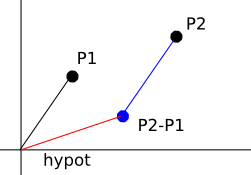
\includegraphics[width=0.4\textwidth]{../img/geom1}
    \end{center}
\end{frame}

\begin{frame}[fragile]{Point Rotation}

  {\smaller

    \begin{exampleblock}{}
\begin{verbatim}
#define PI           3.14159265358979323846  // Pi constant
double PI = 2 * acos(0.0)                    // Better Pi
#define DEG_to_RAD(X) (X*PI)/180.0           // Don't confuse DEG and RAD

// suppose angle t is in degrees (0--360)
point rotate(point p, double t) {
   double rad = DEG_to_RAD(t);
   return point(p.x * cos(rad) - p.y * sin(rad),
                p.x * sin(rad) + p.y * cos(rad));}
\end{verbatim}
    \end{exampleblock}
    \begin{center}
      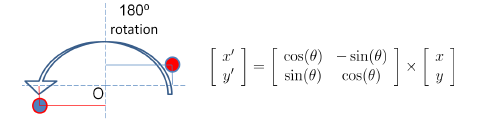
\includegraphics[width=0.8\textwidth]{../img/rotation_halim}
      \ppagenote{Rotation Image from "Competitive Programming 3", Steven Halim}
    \end{center}
}
    {\bf Quiz:} How do you rotate a point around $x_1, y_1$?
\end{frame}

\subsection{Lines}

\begin{frame}[fragile]
  \frametitle{Data Structure for a Line}
  \begin{itemize}
  \item \structure{$ax + by + c = 0$}\hfill (a,b,c) -- useful for most cases
  \item \structure{$y = mx + c$}\hfill (m,c) -- useful for angle manipulation
  \item \structure{$x_0,y_0,x_1,y_1$}\hfill ($p_1, p_2$) -- harder to use, but common input
  \end{itemize}

{\smaller
  \begin{exampleblock}{How to convert from two points to a line}
\begin{verbatim}
struct line { double a,b,c; };

void pointsToLine(point p1, point p2, line &l) {
   if (fabs(p1.x - p2.x) < EPS {
      l.a = 1.0; l.b = 0.0; l.c = -p1.x; }
   else {
      l.a = -(double) (p1.y - p2.y)/(p1.x - p2.x);
      l.b = 1.0; l.c = -(double) (l.a*p1.x) - p1.y;}
}
\end{verbatim}
  \end{exampleblock}
  }
\end{frame}

\begin{frame}[fragile]
  \frametitle{Line Equality}
    \begin{columns}
      \column{0.6\textwidth}
      \begin{itemize}
      \item We define a line as $a,b,c \to (ax+by=c)$

      \item Two lines are parallel if their coefficients $(a, b)$ are the same;\medskip

      \item Two lines are identical if all coefficients $(a,b,c)$ are the same;
      \end{itemize}
      \column{0.4\textwidth}
      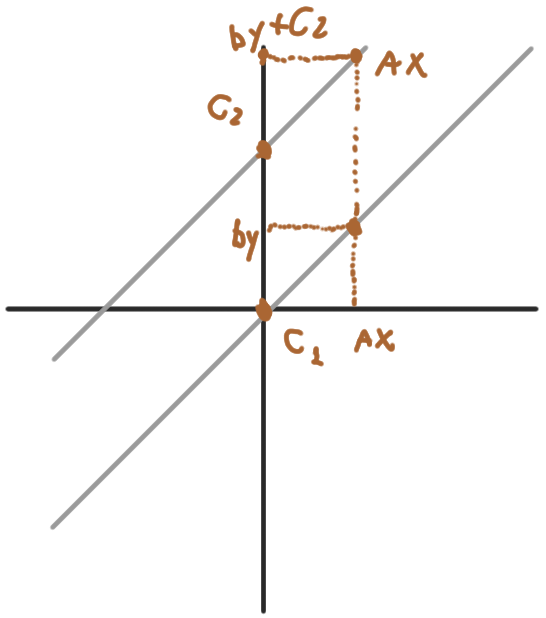
\includegraphics[width=.6\textwidth]{../img/geom3}
    \end{columns}
  \begin{exampleblock}{}
\begin{verbatim}
bool areParallel(line l1, line l2) {
   return (fabs(l1.a-l2.a) < EPS) && (fabs(l1.b-l2.b) < EPS); }

bool areSame(line l1, line l2) {
   return areParallel(l1,l2) && (fabs(l1.c - l2.c) < EPS); }
\end{verbatim}
  \end{exampleblock}
\end{frame}

\begin{frame}[fragile]
  \frametitle{Line Intersection}
    The intersection point $x_I, y_I$ can be found by solving:
    \begin{eqnarray*}
      a_1x_I+b_1y_I+c_1 = 0\\a_2x_I+b_2y_I+c_2 = 0
    \end{eqnarray*}
    Remember that when we create a line $i$, we set $b_i=0$ or $b_i=1$

    {\smaller
    \begin{exampleblock}{}
\begin{verbatim}
bool areIntersect(line l1, line l2, point &p) {
   if (areParallel(l1,l2)) return False;

   p.x = (l2.b * l1.c - l1.b * l2.c) /
         (l2.a * l1.b - l1.a * l2.b);

   // Test for vertical case:
   if (fabs(l1.b) > EPS)     p.y = -(l1.a * p.x + l1.c);
   else                      p.y = -(l2.a * p.x + l2.c);
   return True;
}
\end{verbatim}
    \end{exampleblock}

  }
\end{frame}

\subsection{Segments}
\begin{frame}[fragile]
  \frametitle{Segments and Vectors}
    \begin{columns}
      \column{0.8\textwidth}
      \begin{itemize}
        \item A {\bf line segment} is a line with two endpoints $(p_1, p_2)$;
        \item A {\bf Vector} is a line segment with a direction;
        \begin{itemize}
          \item Represented by its {\bf direction} and {\bf length};
          \item Direction: a point with distance 1 from $(0,0)$
          \item Length: an integer;
          \item Used for movement, translation, speed, etc;
        \end{itemize}
      \end{itemize}
      \column{0.2\textwidth}
      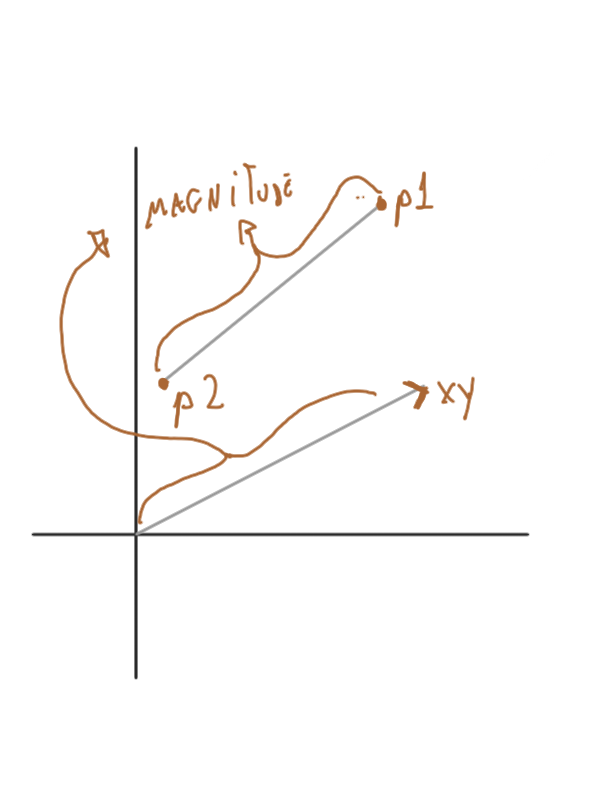
\includegraphics[width=.9\textwidth]{../img/geom4}
    \end{columns}

{\smaller
    \begin{exampleblock}{}
\begin{verbatim}
struct vec { double x, y;
    vec(double _x, double _y) : x(_x), y(_y) {} };

vec toVec(point a, point b) {
    return vec(b.x - a.x, b.y - a.y); }
vec scale(vec v, double s) {
    return vec(v.x * s, v.y * s); }
point translate(point p, vec v) {
    return point(p.x + v.x , p.y + v.y); }
\end{verbatim}
    \end{exampleblock}
  }
\end{frame}

\begin{frame}
  \frametitle{Distance between point and line, point and segment}
  \begin{block}{}
    For a point $p$ and a line $l$ (represented by $\overline{ab}$), the distance between both is given by the segment $pc$, where $c$ is the projection of $p$ in $l$.

    {\smaller
    \begin{columns}[T]
      \column{.5\textwidth}
      Calculating $c$:
      \begin{itemize}
        \item calculate scalar proj. $u$ of $\vec{ap}$ in $l$.
        \item change magnitude of $\vec{ab}$ to $u$ to obtain $\vec{ac}$.
        \item calculate distance between $p$ and $c$.
      \end{itemize}
      \column{.5\textwidth}
      Distance between $p$ and $\overline{ab}$:
      \begin{itemize}
        \item calculate scalar proj. $u$ of $\vec{ap}$ in $l$.
        \item if $u < 0$ or $u > |\vec{ab}|$, then the distance is $\min(d(a,p),d(b,p))$.
        \item else, calculate $\vec{ac}$ and calculate distance $d(p,c)$.
      \end{itemize}
    \end{columns}}
  \end{block}

  \begin{center}
    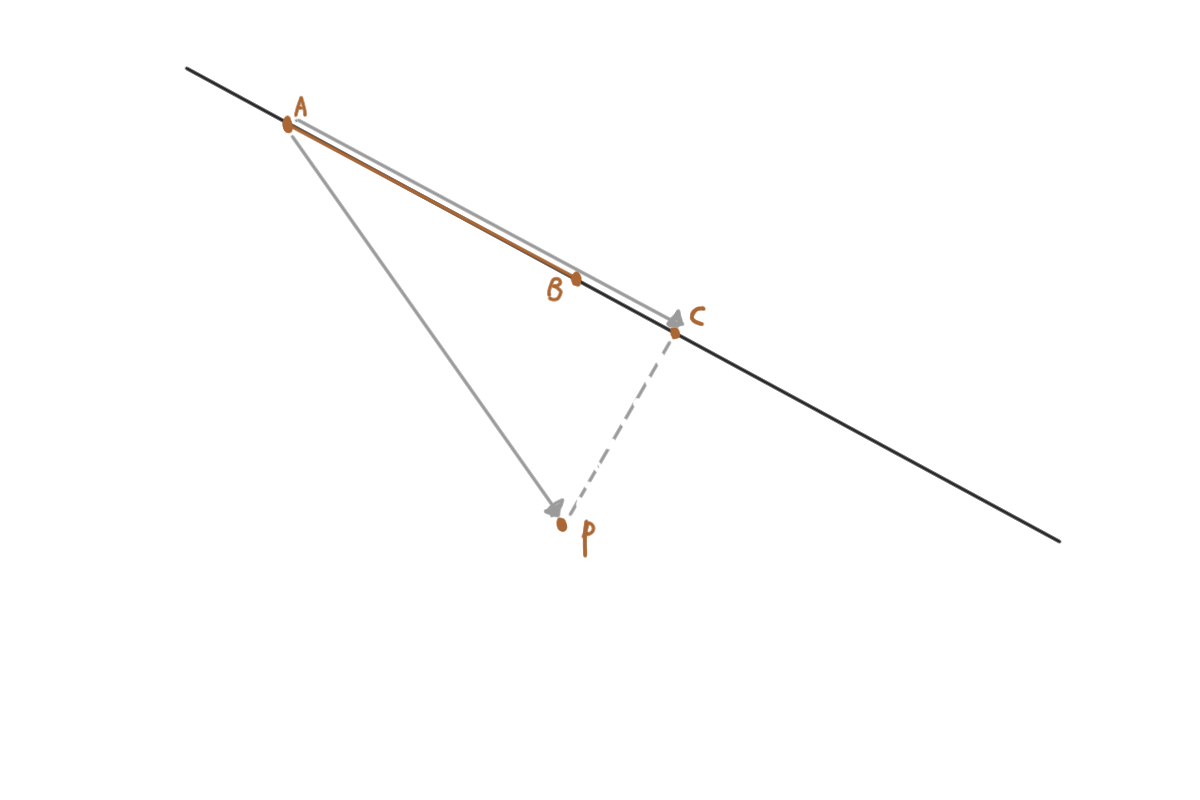
\includegraphics[width=0.5\textwidth]{../img/geom5}
  \end{center}
\end{frame}

\begin{frame}[fragile]
  \frametitle{CODE: Distance between point and line}

  {\smaller
  \begin{exampleblock}{}
\begin{verbatim}
double dot(vec a, vec b) { return (a.x * b.x + a.y * b.y); } // dot product
double norm_sq(vec v) { return v.x * v.x + v.y * v.y; } // norm squared

// Given points a,b,p, calculate distance from p to line ab.
double distToLine(point p, point a, point b, point &c) {
  // point c: c = a + u * |ab|
  vec ap = toVec(a, p), ab = toVec(a, b);

  // dot product calculates size of ap in ab
  // norm square will calculate the scale to ab
  double u = dot(ap, ab) / norm_sq(ab);

  // translate a by u to find point c.
  c = translate(a, scale(ab, u));
  return dist(p, c);
}
\end{verbatim}
  \end{exampleblock}

}
\end{frame}

\begin{frame}[fragile]
  \frametitle{CODE: Distance between point and segment}
  Same as before, but first we test if $c$ is inside $\overline{ab}$.

  {\smaller
    \begin{exampleblock}{}
\begin{verbatim}
double distToSegment(point p, point a, point b, point &c) {
  // next two lines is exact same as last slide
  vec ap = toVec(a, p), ab = toVec(a, b);
  double u = dot(ap, ab) / norm_sq(ab);

  // test if the magnitude $u$ is bigger or smaller than ab.
  if (u < 0.0) { c = point(a.x, a.y); // closer to a
                 return dist(p, a); }
  if (u > 1.0) { c = point(b.x, b.y); // closer to b
                 return dist(p, b); }

  // c is inside AB, same as last slide
  c = translate(a, scale(ab, u));
  return dist(p,c);
}
\end{verbatim}
    \end{exampleblock}
  }
\end{frame}
